\begin{abstract}
Force-plate software reduces each countermovement jump (CMJ) to a few discrete metrics, and athletes with similar values are treated as equivalent. This study examined whether jumps with similar conventional metrics share the same force--time curve, and how much curve-shape variation those metrics capture. In total, \nTrials{} CMJ trials from \nAth{} male footballers (median age \ageMedian{} years), recorded on force plates, were normalised to body weight; the take-off phase and the landing phase, which ended at the lowest point of the centre of mass, were each time-normalised and concatenated. Principal component analysis retained four components that explained \cumFour\% of curve variance, each located almost entirely in the landing phase. Among trials matched on jump height, component-score dispersion was similar to that of the full sample (standard-deviation ratios \jhRatioRange; whole curve \wholeJh), and matching on relative peak force had no effect. Four vendor metrics, age and body mass explained \rtwoRange\% of each component (\cvRange\% under athlete-grouped cross-validation). The first component was most closely related to landing duration ($r$~=~\rLdPCA). Between-athlete differences accounted for \betweenRange\% of component variance. With a fixed 1-s landing window, a take-off component emerged that the metrics largely explained. Equal jump heights conceal different, largely trial-specific landing strategies.
\end{abstract}

\begin{keywords}
countermovement jump; principal component analysis; landing; force--time curve; football
\end{keywords}

\section{Introduction}

The countermovement jump (CMJ) performed on force platforms has become one of the most widely used tests in team sports. It is quick, places little demand on the athlete and is sensitive to training and to neuromuscular fatigue \citep{claudino2017,gathercole2015}. Commercial systems now detect the phases of the jump automatically and return dozens of variables for every trial, among them jump height, peak forces, phase impulses and phase durations \citep{mcmahon2018}. In routine practice, however, decisions rest on a handful of these values. Practitioners are advised to choose a small set of metrics that suits the question being asked, whether it concerns performance profiling, fatigue monitoring or return to sport \citep{bishop2023}. Athletes with similar values on those metrics are then treated, implicitly, as having jumped in a similar way.

That assumption sits uneasily with what is known about movement. The same outcome can be achieved through different coordinative solutions, and variability in how a task is executed is a functional property of the neuromusculoskeletal system rather than mere noise \citep{davids2003,bartlett2007,preatoni2013}. For the vertical jump in particular, no single kinetic or temporal variable fully accounts for performance \citep{dowling1993}. Athletes of different jumping ability differ in how force is distributed across the unweighting, braking and propulsion phases \citep{sole2018}, force--time characteristics differ by sex and sport \citep{laffaye2014}, and the way force is produced within individual sub-phases relates to performance \citep{harry2018}. Performance metrics are increasingly distinguished from strategy variables, such as countermovement depth and phase durations \citep{harry2024}. Analyses of whole force--, velocity-- and power--time curves have described training-induced changes across the curve rather than at single points \citep{cormie2009}, and alternative, strategy-based CMJ variables can detect fatigue when jump height does not \citep{gathercole2015}.

Waveform methods offer a way to describe the whole curve without choosing variables in advance. Principal component analysis (PCA) of time-normalised waveforms, and its functional counterpart, decompose a set of curves into a small number of orthogonal modes of variation, each with a score for every trial \citep{jolliffe2002,ramsay2005,jolliffe2016}. In biomechanics these methods have described gait waveforms associated with knee osteoarthritis \citep{deluzio2007}, knee kinematics in the vertical jump \citep{ryan2006}, running kinematics in Achilles tendinopathy \citep{donoghue2008} and on-water rowing \citep{warmenhoven2019}, and principled ways of interpreting the components have been proposed \citep{brandon2013}. For vertical jumps, dimensionality-reduction techniques describe performance-related aspects of the curve better than discrete points do \citep{richter2014b}, principal component waveform analysis identifies improvements in jump performance \citep{floria2019}, and alignment of the curves on biomechanical events improves the information that can be extracted from them \citep{richter2014a,moudy2018}.

Two gaps remain. First, the landing that follows every CMJ is usually discarded, even though it is recorded on the same plates in the same trial. Landing kinetics are of independent interest: stiff landings with high vertical forces have been associated with anterior cruciate ligament injury risk in young female athletes \citep{leppanen2017}, jumping and landing variables have some utility as predictors of injury \citep{pedley2020}, and CMJ landing characteristics change with the effort that athletes perceive themselves to be making \citep{hite2025}. Second, although waveform studies show that curves carry information beyond discrete variables, the extent to which the metrics reported in routine monitoring fail to capture curve shape has rarely been quantified directly, and never, to our knowledge, by asking whether jumps matched on those metrics have matched curves. Routinely collected data from youth football, in which large numbers of tests are performed under field conditions, provide an opportunity to answer this question on a realistic scale.

The present study therefore analysed the concatenated take-off and landing force--time curves of male footballers, with three aims: (i) to identify the principal modes of variation of the curve and to interpret them biomechanically; (ii) to test whether trials matched on jump height, or on relative concentric peak force, show less curve-shape variation than the sample as a whole; and (iii) to quantify how much of each mode of variation is explained by four conventional vendor metrics together with age and body mass, using evaluation schemes that respect the repeated trials of each athlete. In addition, the partition of curve-shape variation between athletes, sessions and trials, and the sensitivity of the conclusions to the definition of the landing phase, were examined.

\section{Materials and methods}

\subsection{Study design and overview}

This was a retrospective, cross-sectional analysis of routinely collected force-plate data. The analysis followed the pipeline in Figure~\ref{fig:pipeline}. Quality-control rules, phase definitions, the number of retained components and the matched-band definition were fixed before any result was examined; the analysis does not include any data-driven tuning of these choices.

\begin{figure}[htbp]
\centering
\resizebox{\textwidth}{!}{% Pipeline flow diagram (Figure 1); used in the manuscript and compiled standalone for the submission file
\begin{tikzpicture}[
  node distance=2.6mm and 4mm,
  box/.style={draw, rounded corners=1.5pt, align=flush left, font=\sffamily\scriptsize, text width=52mm, inner sep=3pt, fill=#1},
  box/.default=white,
  arr/.style={-{Stealth[length=1.6mm]}, thick, gray!70!black}]
\node[box=blue!6] (b1) {\textbf{1. Data}\\ Routine VALD ForceDecks CMJ tests, male footballers; dual-plate vertical force (1000\,Hz; 60 trials at 500\,Hz) and vendor trial metrics; pseudonymous codes};
\node[box=blue!6, below=of b1] (b2) {\textbf{2. Events and phases}\\ vendor onset, take-off and touch-down; take-off phase = onset $\rightarrow$ take-off; landing phase = touch-down $\rightarrow$ lowest centre of mass (velocity $=0$), or touch-down $+1$\,s (sensitivity)};
\node[box=blue!6, below=of b2] (b3) {\textbf{3. Quality control}\\ R1 valid body mass; R2 quiet-stance mass within 5\%; R3 flight force $\le 50$\,N; R4 complete metrics and age; R5 lowest centre of mass found};
\node[box=green!7, below=of b3] (b4) {\textbf{4. Curve construction}\\ force $\div$ body weight; each phase resampled to 101 points; phases concatenated without flight $\rightarrow$ 202-point curve};
\node[box=orange!9, right=of b1] (b5) {\textbf{5. Aim 1: modes of variation}\\ covariance PCA (centred, unscaled); four components retained a priori; mean $\pm 2$\,SD reconstructions; loading share by phase; correlations with descriptors};
\node[box=orange!9, below=of b5] (b6) {\textbf{6. Aim 2: matched-band dispersion}\\ trials in the 45th--55th percentile of jump height or relative peak force; SD ratio band / full sample; athlete bootstrap 95\% CI};
\node[box=orange!9, below=of b6] (b7) {\textbf{7. Aim 3: variance explained}\\ OLS of each score on four vendor metrics, age and body mass; $R^2$ in-sample, athlete-grouped 5-fold CV, one trial per athlete, athlete means};
\node[box=red!6, below=of b7] (b8) {\textbf{8. Structure and sensitivity}\\ athlete / session / trial variance decomposition; 1-s landing window; matched-band width};
\draw[arr] (b1) -- (b2); \draw[arr] (b2) -- (b3); \draw[arr] (b3) -- (b4);
\draw[arr] (b4.east) -- ++(2mm,0) |- (b5.west);
\draw[arr] (b5) -- (b6); \draw[arr] (b6) -- (b7); \draw[arr] (b7) -- (b8);
\end{tikzpicture}
}
\caption{\capPipeline}
\label{fig:pipeline}
\end{figure}


\subsection{Participants and data source}

Data were countermovement jumps performed by male football players during routine testing at a high-performance centre in Thane, Mumbai, India \todo{name or describe the centre or programme, the testing period, and the data-sharing agreement}. All CMJ trials of male football players available through the VALD ForceDecks external application programming interface were extracted (\nTrialsAll{} trials from \nAthAll{} athletes in \nSessAll{} sessions). Before analysis, athletes, tests and trials were replaced by pseudonymous codes; the analysis files contain no names, team names, dates of birth, test dates or vendor identifiers, and the key linking codes to athletes is held separately by the first author. Age at test was computed before de-identification and rounded to 0.1 year. Of the \nAth{} analysed athletes, \nMinors{} (\pctMinors\%) were under 18 years of age at their first analysed test. \todo{ethics committee, approval number, consent of athletes and parental or guardian consent for those under 18 years, or the waiver of consent for the secondary use of routine monitoring data, and a statement that the study conformed to the Declaration of Helsinki}.

\subsection{Instrumentation and test protocol}

Trials were recorded on VALD ForceDecks dual force platforms (VALD Performance, Brisbane, Australia), which record the vertical ground reaction force under each foot. Total vertical force was the sum of the two plates. Most trials were sampled at 1000\,Hz; \nFsLow{} trials were recorded at 500\,Hz, which does not affect the analysis because every phase was resampled to a common grid (Section~\ref{sec:curves}). Each session contained one or more trials (median \trialsPerSessMedian{} per session), and athletes contributed a median of \sessPerAthMedian{} session (maximum \sessPerAthMax). \todo{warm-up, instructions given to athletes (including arm position and landing instructions), number of trials requested, rest between trials, and the criteria used by the testers to accept a trial}. The vendor software identified movement onset and returned, for every trial, the four metrics used in this study: jump height (from flight time), concentric peak force, eccentric braking impulse and concentric impulse over the first 100\,ms of the concentric phase, together with contraction time, flight time, countermovement depth and peak landing force, which were used only for interpretation.

\subsection{Event detection and phase definitions}
\label{sec:events}

Three events were taken from the vendor output: movement onset $t_{\mathrm{on}}$, take-off $t_{\mathrm{to}} = t_{\mathrm{on}} + T_{\mathrm{c}}$, where $T_{\mathrm{c}}$ is the contraction time, and touch-down $t_{\mathrm{td}} = t_{\mathrm{to}} + T_{\mathrm{f}}$, where $T_{\mathrm{f}}$ is the flight time \citep{owen2014,mcmahon2018,harry2020}. The take-off phase ran from $t_{\mathrm{on}}$ to $t_{\mathrm{to}}$. In the main analysis the landing phase ran from touch-down to the lowest point of the centre of mass (COM), the instant at which the downward velocity acquired during the fall is first brought to zero, which marks the end of impact absorption. The vertical velocity of the COM was obtained by integrating the impulse--momentum relationship from touch-down \citep{linthorne2001,street2001},
\begin{equation}
v(t) = -\frac{g\,T_{\mathrm{f}}}{2} + \int_{t_{\mathrm{td}}}^{t} \frac{F(s) - m g}{m}\,\mathrm{d}s,
\qquad
t_{\mathrm{lc}} = \min\{\, t > t_{\mathrm{td}} : v(t) \ge 0 \,\},
\label{eq:velocity}
\end{equation}
where $F$ is the total vertical force, $m$ the body mass, $g = 9.81$\,m\,s$^{-2}$ and the initial value is the touch-down velocity implied by a symmetrical flight. The landing phase in the main analysis was $[t_{\mathrm{td}}, t_{\mathrm{lc}}]$. Because no consensus definition of the end of the CMJ landing exists, a sensitivity analysis used a fixed window from touch-down to 1\,s after touch-down, which is the end of the vendor's trial record.

\subsection{Quality control}

Five rules were applied in order (Table~\ref{tab:qc}). Trials were excluded if the vendor body mass was missing or invalid (R1), because every curve is divided by body weight; if the mass estimated from quiet stance before the jump differed from the vendor body mass by more than 5\% (R2), which indicates an incorrectly entered mass or an athlete who was not still; if the mean force recorded during flight exceeded 50\,N (R3), which indicates contact with the plate during flight or an event-detection error; if any of the four metrics or age was missing (R4); or, in the main analysis only, if the lowest point of the COM could not be identified within the recorded landing (R5).

\begin{table}[htbp]
\tbl{Quality-control flow (main analysis).}
{\small\begin{tabular}{lrrr}
\toprule
Step & Trials & Sessions & Athletes \\
\midrule
All male football CMJ trials & 833 & 333 & 215 \\
R1: valid body mass & 828 & 329 & 212 \\
R2: quiet-stance mass within 5% of body mass & 813 & 328 & 212 \\
R3: no force on plate during flight & 811 & 327 & 212 \\
R4: complete metrics and age & 811 & 327 & 212 \\
R5: end of landing (lowest COM) found & 805 & 327 & 212 \\
\bottomrule
\end{tabular}
}
\tabnote{Rules R1--R4 were fixed before any result was examined; R5 applies only to the main landing definition (touch-down to the lowest point of the centre of mass), and the 1-s landing window therefore retained \nTrialsS{} trials. Sessions, test occasions on which an athlete performed one or more trials. COM, centre of mass.}
\label{tab:qc}
\end{table}


\subsection{Curve construction}
\label{sec:curves}

Force was expressed in multiples of body weight, $\tilde F(t) = F(t)/(m g)$, so that curves of athletes of different mass are directly comparable and a value of one corresponds to quiet standing. Each phase $[t_a, t_b]$ was then resampled by linear interpolation at 101 equally spaced instants,
\begin{equation}
\tilde F^{(p)}_k = \tilde F\!\left(t_a + \tfrac{k}{100}\,(t_b - t_a)\right), \qquad k = 0, 1, \ldots, 100,
\end{equation}
which aligns take-off at the end of the first block and touch-down at the start of the second, a simple form of landmark registration \citep{ramsay2005,richter2014a,moudy2018}. Time-normalising the whole trial to a single scale was rejected because the same event would then fall at different percentages in different trials, and timing differences would be confounded with differences in shape. The flight phase was omitted: during flight the force is zero, so this portion of the curve carries no information about force production except its duration, which determines flight-time jump height \citep{linthorne2001}; retaining it would allow the analysis to recover a conventional metric from the length of a block. Each trial was therefore represented by the vector $\mathbf{x}_i \in \mathbb{R}^{202}$ formed by the take-off block followed by the landing block.

\subsection{Principal component analysis}

PCA was applied to the $n \times 202$ matrix of curves \citep{jolliffe2002,jolliffe2016}. Because all points share the same unit, the analysis used the covariance matrix of the centred curves, without scaling,
\begin{equation}
\mathbf{S} = \frac{1}{n-1}\sum_{i=1}^{n}(\mathbf{x}_i - \bar{\mathbf{x}})(\mathbf{x}_i - \bar{\mathbf{x}})^{\top} = \mathbf{V}\boldsymbol{\Lambda}\mathbf{V}^{\top},
\qquad
z_{ik} = \mathbf{v}_k^{\top}(\mathbf{x}_i - \bar{\mathbf{x}}),
\end{equation}
where $\mathbf{v}_k$ is the $k$th loading vector (unit length), $\lambda_k$ its eigenvalue and $z_{ik}$ the score of trial $i$ on component $k$; the proportion of variance explained by component $k$ is $\lambda_k / \sum_j \lambda_j$. Four components were retained, as specified before the analysis. The sign of each loading vector was fixed so that its largest absolute element was positive. Components were interpreted in three ways: by reconstructing the curves $\bar{\mathbf{x}} \pm 2\sqrt{\lambda_k}\,\mathbf{v}_k$, which show the effect of a two-standard-deviation change in the score \citep{brandon2013,warmenhoven2019}; by the share of each component located in the landing phase, $\sum_{j \in \mathcal{L}} v_{jk}^2$, where $\mathcal{L}$ indexes the 101 landing points; and by Pearson correlations of the scores with interpretable descriptors (peak landing force relative to body weight, landing duration $t_{\mathrm{lc}} - t_{\mathrm{td}}$, contraction time, countermovement depth, the four vendor metrics, age and body mass).

\subsection{Matched-band dispersion}

To test whether equal conventional scores imply equal curves (aim ii), trials between the 45th and 55th percentiles of jump height were selected, and, separately, trials between the same percentiles of concentric peak force relative to body weight. For each component, the dispersion ratio
\begin{equation}
\rho_k = \frac{\mathrm{SD}(z_{k} \mid i \in \mathcal{B})}{\mathrm{SD}(z_{k})}
\end{equation}
compares the standard deviation of the score among trials in band $\mathcal{B}$ with that in the full sample. A ratio close to one indicates that fixing the metric does not make curves more alike; a ratio well below one indicates that the metric constrains curve shape. The same comparison was made for the whole curve as $\rho = \{\mathrm{tr}(\mathbf{S}_{\mathcal{B}})/\mathrm{tr}(\mathbf{S})\}^{1/2}$, where $\mathbf{S}_{\mathcal{B}}$ is the covariance matrix within the band. Because athletes contributed several trials, 95\% confidence intervals for $\rho_k$ were obtained from \nBoot{} bootstrap resamples of athletes, each resample including all trials of the selected athletes, with band limits held fixed \citep{efron1993}.

\subsection{Variance explained by conventional metrics}

For aim (iii), each component score was regressed by ordinary least squares on the four vendor metrics and on age and body mass,
\begin{equation}
z_{ik} = \beta_{0k} + \sum_{q=1}^{6}\beta_{qk}\,w_{iq} + \varepsilon_{ik},
\end{equation}
and the coefficient of determination $R^2_k$ was taken as the share of the component explained; $1 - R^2_k$ is the share left unexplained. Because in-sample $R^2$ is optimistic and trials of the same athlete are not independent, three further evaluations were made. In athlete-grouped five-fold cross-validation, athletes rather than trials were allocated to folds \citep{roberts2017}, and the out-of-sample coefficient was computed as $1 - \sum_i (z_{ik} - \hat z^{(-f)}_{ik})^2 / \sum_i (z_{ik} - \bar z_k)^2$, where $\hat z^{(-f)}_{ik}$ is the prediction from the model fitted without the fold containing trial $i$. The regressions were also refitted with one randomly selected trial per athlete and with athlete means of all variables.

\subsection{Structure of repeated measurements}

To establish whether component scores describe stable characteristics of athletes or vary from trial to trial, each score was decomposed with a three-level random-intercept model,
\begin{equation}
z_{ajt} = \mu + a_a + b_{aj} + e_{ajt}, \quad a_a \sim N(0, \sigma^2_{\mathrm{A}}),\; b_{aj} \sim N(0, \sigma^2_{\mathrm{S}}),\; e_{ajt} \sim N(0, \sigma^2_{\mathrm{T}}),
\end{equation}
for trial $t$ of session $j$ of athlete $a$, fitted by restricted maximum likelihood \citep{pinheiro2000}. The shares $\sigma^2_{\mathrm{A}}$, $\sigma^2_{\mathrm{S}}$ and $\sigma^2_{\mathrm{T}}$ of the total variance were reported; the between-athlete share is an intraclass correlation coefficient for a single trial \citep{hopkins2000,koo2016}.

\subsection{Sensitivity analyses}

The complete analysis was repeated with the 1-s landing window. The width of the jump-height band was varied (40th--60th percentile, and median $\pm$ 1\,cm and $\pm$ 2\,cm).

\subsection{Software and reproducibility}

All analyses were run by a single R script in R 4.5.3 \citep{rcore2026} with the packages dplyr, tidyr, ggplot2 \citep{wickham2016}, patchwork and nlme \citep{pinheiro2000}; every random step (cross-validation folds, the one-trial selection and the bootstrap) used seed \seedValue. The script writes every table, figure and number reported in this article. A preliminary version of this analysis was summarised in a conference report; rerunning the script from the de-identified data reproduced all \nReproTotal{} values checked against that report. Statistical reporting followed recommendations for sports medicine and exercise science \citep{hopkins2009}. \todo{repository URL or DOI once public}.

\section{Results}

\subsection{Sample}

Of \nTrialsAll{} trials, \nTrials{} trials from \nAth{} athletes in \nSess{} sessions met all quality-control criteria (Table~\ref{tab:qc}); the 1-s landing window retained \nTrialsS{} trials, because the lowest point of the COM could not be identified in \nLowcomMissing{} trials. Athletes were \ageMedian{} years of age at their first analysed test (median; interquartile range \ageQone--\ageQthree{}; range \ageMin--\ageMax) and contributed \trialsPerAthMean{} trials on average (maximum \trialsPerAthMax). Mean jump height was \jhMean{} $\pm$ \jhSD{}\,cm, and peak landing force ranged from \lpfMin{} to \lpfMax{} times body weight (Table~\ref{tab:desc}).

\begin{table}[htbp]
\tbl{Characteristics of the analysed sample (\nTrials{} trials, \nAth{} athletes).}
{\scriptsize\setlength{\tabcolsep}{4pt}\begin{tabular}{lrlll}
\toprule
Variable & $n$ & Mean $\pm$ SD & Median (IQR) & Range \\
\midrule
Age at first test (years) & 212 & 16.01 $\pm$ 5.94 & 14.10 (12.00 to 16.80) & 8.80 to 37.90 \\
Body mass at first test (kg) & 212 & 53.31 $\pm$ 15.90 & 51.73 (40.86 to 64.03) & 25.03 to 95.97 \\
Jump height, flight time (cm) & 805 & 28.19 $\pm$ 8.43 & 26.96 (21.62 to 34.69) & 8.54 to 51.47 \\
Concentric peak force (N) & 805 & 1269.26 $\pm$ 420.74 & 1227.01 (923.47 to 1582.99) & 473.52 to 3073.22 \\
Concentric peak force ($\times$\,BW) & 805 & 2.35 $\pm$ 0.38 & 2.29 (2.11 to 2.51) & 1.65 to 4.70 \\
Eccentric braking impulse (N\,s) & 805 & 27.80 $\pm$ 15.43 & 24.60 (16.59 to 35.70) & 0.00 to 95.18 \\
Concentric impulse, first 100 ms (N\,s) & 805 & 62.24 $\pm$ 26.66 & 58.70 (41.76 to 79.14) & 1.51 to 187.93 \\
Peak landing force ($\times$\,BW) & 805 & 5.39 $\pm$ 1.97 & 4.97 (3.88 to 6.67) & 2.19 to 14.88 \\
Contraction time (s) & 805 & 0.78 $\pm$ 0.19 & 0.77 (0.66 to 0.90) & 0.31 to 1.48 \\
Countermovement depth (cm) & 805 & $-$26.55 $\pm$ 9.90 & $-$27.13 ($-$33.55 to $-$20.71) & $-$52.39 to 0.00 \\
Touch-down to lowest COM (s) & 805 & 0.25 $\pm$ 0.11 & 0.24 (0.15 to 0.31) & 0.07 to 0.93 \\
Trials per athlete & 212 & 3.80 $\pm$ 2.28 & 3.00 (2.00 to 5.00) & 1.00 to 16.00 \\
Trials per session & 327 & 2.46 $\pm$ 0.78 & 2.00 (2.00 to 3.00) & 1.00 to 7.00 \\
Sessions per athlete & 212 & 1.54 $\pm$ 0.80 & 1.00 (1.00 to 2.00) & 1.00 to 6.00 \\
\bottomrule
\end{tabular}
}
\tabnote{Age and body mass are per athlete at the first analysed trial; all other rows are per trial unless stated. Jump height, from flight time. Countermovement depth is the vendor estimate of centre-of-mass displacement (negative downwards). Touch-down to lowest COM, duration of the landing phase in the main analysis. BW, body weight; COM, centre of mass; IQR, interquartile range.}
\label{tab:desc}
\end{table}


\subsection{Modes of variation of the force--time curve (aim i)}

The mean curve showed the expected unweighting, braking and propulsion pattern in the take-off phase and a large, variable force peak in the landing phase (Figure~\ref{fig:mean}A). Point-wise dispersion was much greater during landing than during take-off. The first component explained \varPCA\% of the variance, and the four retained components together explained \cumFour\% (Figure~\ref{fig:mean}B); ten components were needed to explain \cumTen\%.

\begin{figure}[htbp]
\centering
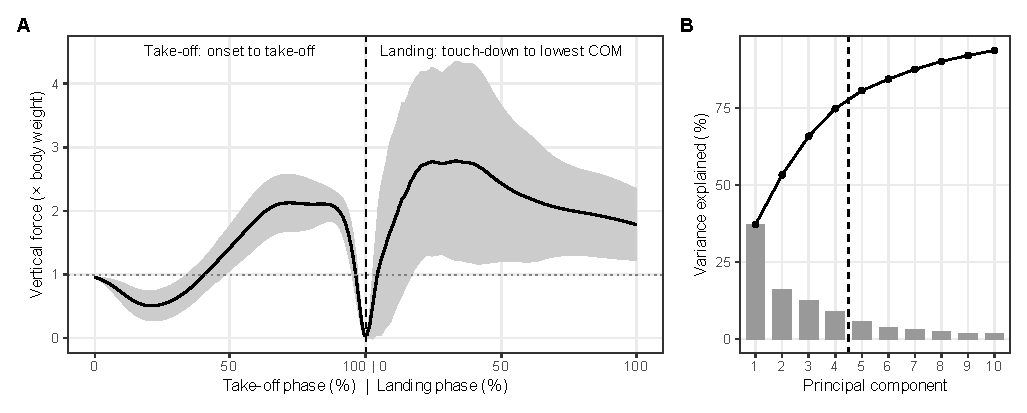
\includegraphics[width=\textwidth]{Fig2_mean_curve_scree.pdf}
\caption{\capMean}
\label{fig:mean}
\end{figure}


All four retained components were located almost entirely in the landing phase, which held \ldsPCD--\ldsPCB\% of their squared loadings (Table~\ref{tab:pcs}). PC1 (\varPCA\%) contrasted landings in which force rose to a large peak at about \peakPCA\% of the landing phase and remained well above body weight until the lowest point of the COM with landings in which force peaked early and then declined (Figure~\ref{fig:pcs}). Its strongest correlate was landing duration ($r$~=~\rLdPCA): high scores denote short, stiff landings in which the downward momentum is arrested quickly. PC1 was moderately related to peak landing force ($r$~=~\rLpfPCA) and essentially unrelated to contraction time ($r$~=~\rCtPCA) and countermovement depth ($r$~=~\rCmdPCA). PC2 to PC4 (\varPCB\%, \varPCC\% and \varPCD\%) described the timing and number of landing force peaks, contrasting single early peaks, single later peaks and double-peaked landings, with their largest loadings at \peakPCB\%, \peakPCC\% and \peakPCD\% of the landing phase. Peak landing force correlated with every component ($r$ = \lpfCorRange), whereas the correlations with contraction time and countermovement depth did not exceed \ctAbsMax{} and \cmdAbsMax{} in absolute value, and those with the vendor metrics did not exceed \vendorAbsMax.

\begin{table}[htbp]
\tbl{Retained principal components of the concatenated take-off and landing curve (main analysis).}
{\scriptsize\setlength{\tabcolsep}{3.5pt}\begin{tabular}{lrrrlrrrrr}
\toprule
 & Variance & Cumulative & Landing share & Largest & \multicolumn{5}{c}{Pearson $r$ with} \\
\cmidrule(l){6-10}
Component & (\%) & (\%) & of loading (\%) & loading at & LPF & JH & CT & CMD & LD \\
\midrule
PC1 & 37.3 & 37.3 & 99.7 & Landing 40\% & 0.39 & 0.13 & $-$0.04 & 0.01 & $-$0.75 \\
PC2 & 16.0 & 53.3 & 99.9 & Landing 26\% & 0.22 & 0.13 & 0.02 & 0.00 & $-$0.14 \\
PC3 & 12.6 & 65.9 & 99.5 & Landing 16\% & 0.39 & 0.34 & 0.00 & $-$0.14 & $-$0.32 \\
PC4 & 8.9 & 74.8 & 99.3 & Landing 9\% & 0.45 & 0.24 & 0.15 & $-$0.18 & $-$0.04 \\
\bottomrule
\end{tabular}
}
\tabnote{Landing share of loading, percentage of the squared loading vector that falls in the landing block (the remainder falls in the take-off block). Largest loading at, phase and percentage of the phase at which the loading has its largest absolute value. LPF, peak landing force (\,$\times$\,BW); JH, jump height; CT, contraction time; CMD, countermovement depth; LD, landing duration (touch-down to lowest COM). Signs are fixed so that the largest absolute loading is positive.}
\label{tab:pcs}
\end{table}

\begin{figure}[htbp]
\centering
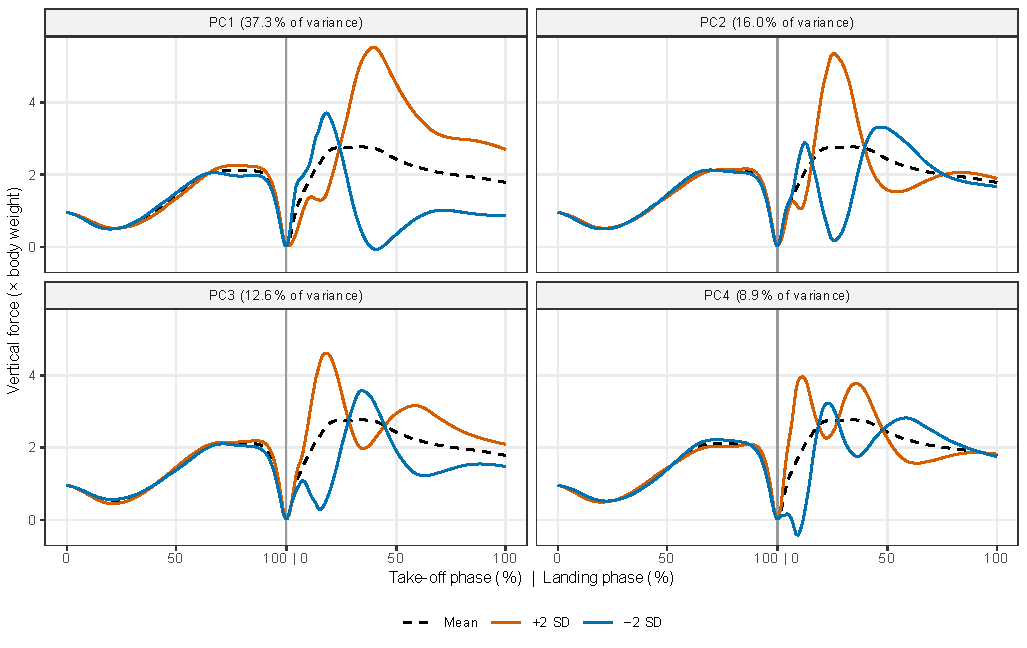
\includegraphics[width=\textwidth]{Fig3_pc_reconstructions_main.pdf}
\caption{\capPCs}
\label{fig:pcs}
\end{figure}


\subsection{Curve shape among trials matched on conventional metrics (aim ii)}

The jump-height band contained \jhBandN{} trials from \jhBandAth{} athletes with a jump height of \jhBandMean{} $\pm$ \jhBandSD{}\,cm, a standard deviation \jhBandSDfactor{} times smaller than that of the full sample. Within this band, take-off curves were similar but landing curves differed widely (Figure~\ref{fig:band}A). Matching on jump height reduced the dispersion of PC1 only modestly (ratio \jhRatioPCA, 95\% CI \jhLoPCA--\jhHiPCA), and the ratios for the other components ranged from \jhRatioOtherRange; every confidence interval included one (Table~\ref{tab:band}, Figure~\ref{fig:band}B). The dispersion of the whole curve was unchanged (ratio \wholeJh). Matching on relative concentric peak force had no discernible effect (component ratios \rpfRatioRange; whole curve \wholeRpf). The result did not depend on the width of the band: across four band definitions the PC1 ratio ranged from \bwPCARange, and all ratios from \bwAllRange.

\begin{table}[htbp]
\tbl{Dispersion of component scores in the full sample and among trials matched on jump height or on relative concentric peak force (main analysis).}
{\scriptsize\setlength{\tabcolsep}{4pt}\begin{tabular}{lrrlrl}
\toprule
 & SD, full & \multicolumn{2}{c}{Jump-height band} & \multicolumn{2}{c}{Relative peak-force band} \\
\cmidrule(lr){3-4}\cmidrule(l){5-6}
Component & sample & SD & Ratio (95\% CI) & SD & Ratio (95\% CI) \\
\midrule
PC1 & 7.28 & 6.45 & 0.89 (0.70--1.06) & 7.33 & 1.01 (0.77--1.16) \\
PC2 & 4.77 & 4.62 & 0.97 (0.77--1.16) & 5.01 & 1.05 (0.82--1.24) \\
PC3 & 4.22 & 4.03 & 0.95 (0.74--1.13) & 4.25 & 1.00 (0.81--1.17) \\
PC4 & 3.56 & 4.16 & 1.17 (0.81--1.44) & 3.75 & 1.05 (0.87--1.23) \\
Whole curve$^a$ & 11.92 & 11.99 & 1.01 & 11.95 & 1.00 \\
\bottomrule
\end{tabular}
}
\tabnote{Matched bands comprise trials between the 45th and 55th percentiles of jump height (\jhBandLo--\jhBandHi\,cm; \jhBandN{} trials, \jhBandAth{} athletes) or of concentric peak force relative to body weight (\rpfBandLo--\rpfBandHi\,BW; \rpfBandN{} trials, \rpfBandAth{} athletes). Ratio, SD in the band divided by SD in the full sample; 95\% CI from \nBoot{} athlete-level bootstrap resamples. Component SDs depend on the number of grid points and are comparable only within this table; ratios are scale-free. $^a$Square root of the summed point-wise variance of the 202-point curve.}
\label{tab:band}
\end{table}

\begin{figure}[htbp]
\centering
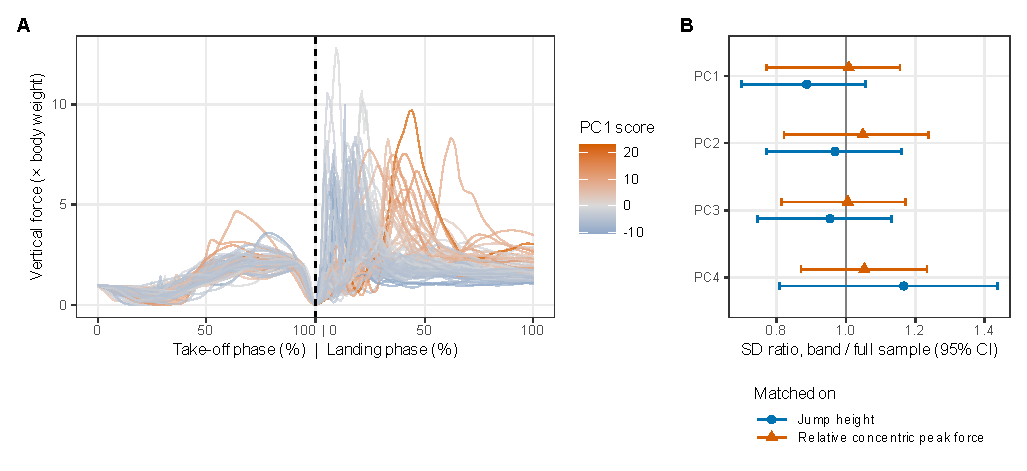
\includegraphics[width=\textwidth]{Fig4_matched_band.pdf}
\caption{\capBand}
\label{fig:band}
\end{figure}


\subsection{Variance explained by conventional metrics (aim iii)}

The four vendor metrics, age and body mass explained \rtwoRange\% of the variance of the retained components, leaving \unexplRange\% unexplained (Table~\ref{tab:r2}, Figure~\ref{fig:r2}). Explained variance was lower under athlete-grouped cross-validation (\cvRange\%), and similar when one trial per athlete (\oneTrialRange\%) or athlete means (\athMeanRange\%) were analysed, so the low values were not a consequence of treating repeated trials as independent.

\begin{table}[htbp]
\tbl{Variance of each component score explained by the four vendor metrics, age and body mass, and decomposition of component-score variance (main analysis).}
{\scriptsize\setlength{\tabcolsep}{3.2pt}\begin{tabular}{lrrrrrrrr}
\toprule
 & \multicolumn{5}{c}{$R^2$ of component score on metrics, age and body mass (\%)} & \multicolumn{3}{c}{Variance of component score (\%)} \\
\cmidrule(lr){2-6}\cmidrule(l){7-9}
Component & In-sample & Adjusted & Athlete CV & One trial & Athlete & Between & Between & Within \\
 & & & & per athlete & means & athletes & sessions & session \\
\midrule
PC1 & 7.7 & 7.0 & 4.0 & 10.0 & 11.1 & 29.6 & 34.9 & 35.5 \\
PC2 & 2.7 & 2.0 & 0.3 & 4.3 & 5.4 & 21.4 & 17.0 & 61.6 \\
PC3 & 13.1 & 12.4 & 11.8 & 17.8 & 21.2 & 22.9 & 2.3 & 74.8 \\
PC4 & 9.1 & 8.4 & 6.3 & 11.1 & 13.8 & 10.0 & 20.3 & 69.6 \\
\bottomrule
\end{tabular}
}
\tabnote{Predictors: jump height, concentric peak force, eccentric braking impulse, concentric impulse over the first 100\,ms, age and body mass (ordinary least squares). In-sample and adjusted, all \nTrials{} trials. Athlete CV, out-of-sample $R^2$ from five-fold cross-validation with athletes, not trials, allocated to folds. One trial per athlete, one randomly drawn trial per athlete (\nAth{} trials). Athlete means, scores and predictors averaged within athlete. Variance shares from a three-level random-intercept model (athlete, session within athlete, trial within session) fitted by restricted maximum likelihood.}
\label{tab:r2}
\end{table}


Between-athlete differences accounted for \betweenRange\% of the variance of the component scores, differences between sessions of the same athlete for \sessRange\%, and differences between trials within a session for \withinRange\% (Table~\ref{tab:r2}). PC1 was the most athlete-specific component (\betweenPCA\% between athletes, \sessPCA\% between sessions); for PC2 to PC4, \withinPCB\%, \withinPCC\% and \withinPCD\% of the variance arose between trials of the same session.

\begin{figure}[htbp]
\centering
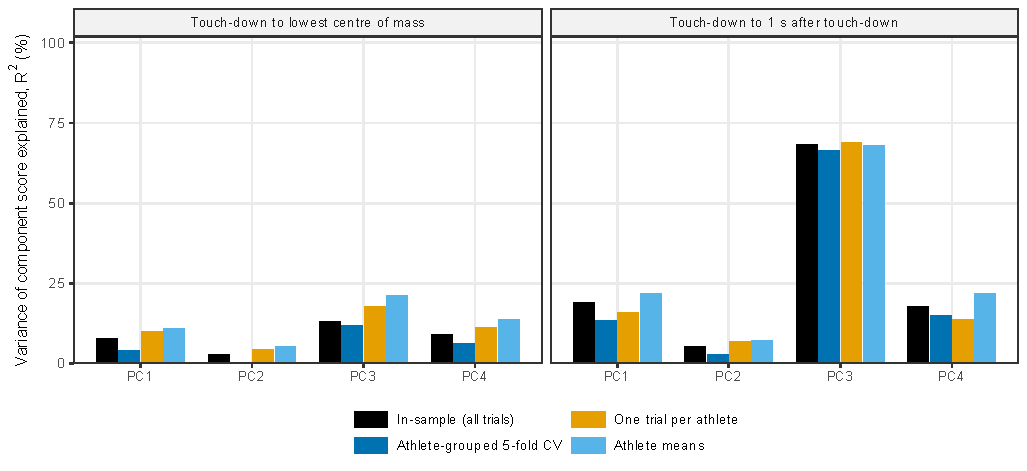
\includegraphics[width=\textwidth]{Fig5_variance_explained.pdf}
\caption{\capRtwo}
\label{fig:r2}
\end{figure}


\subsection{Sensitivity to the definition of the landing phase}

With the landing phase ending 1\,s after touch-down, the impact occupied only the first few per cent of the landing block and the remainder approximated quiet standing (Figure~\ref{fig:window}). The four components then explained \cumFourS\% of the variance, and PC3 became a take-off component (\ldsSPCCtakeoff\% of its squared loading in the take-off phase) that was strongly related to contraction time ($r$~=~\rCtSPCC) and relative concentric peak force ($r$~=~\rRpfSPCC). This component was largely explained by the conventional metrics ($R^2$ = \rtwoSPCC\%; \cvSPCC\% under cross-validation), whereas the three landing components remained poorly explained ($R^2$ = \rtwoLandingSRange\%; Table~\ref{tab:window}, Figure~\ref{fig:r2}). PC1 was again a landing component related to peak landing force ($r$~=~\rLpfSPCA) and landing duration ($r$~=~\rLdSPCA). Matching on jump height reduced PC1 dispersion somewhat more under this definition (ratio \jhRatioSPCA, 95\% CI \jhLoSPCA--\jhHiSPCA), but the dispersion of the whole curve was again unchanged (ratio \wholeJhS).

\begin{table}[htbp]
\tbl{Main analysis compared with the sensitivity analysis in which the landing phase ended 1\,s after touch-down.}
{\scriptsize\setlength{\tabcolsep}{4pt}\begin{tabular}{lll}
\toprule
Quantity & Main: landing to lowest COM & Sensitivity: 1-s landing \\
\midrule
Trials / athletes after QC & 805 / 212 & 811 / 212 \\
Variance explained, PC1--PC4 (\%) & 37.3, 16.0, 12.6, 8.9 & 20.2, 16.6, 15.1, 10.2 \\
Cumulative, PC1--PC4 (\%) & 74.8 & 62.2 \\
Landing share of loading, PC1--PC4 (\%) & 99.7, 99.9, 99.5, 99.3 & 96.4, 92.5, 3.7, 80.2 \\
PC1 SD ratio, jump-height band (95\% CI) & 0.89 (0.70--1.06) & 0.82 (0.69--0.96) \\
Whole-curve SD ratio, jump-height band & 1.01 & 1.01 \\
In-sample $R^2$, PC1--PC4 (\%) & 7.7, 2.7, 13.1, 9.1 & 19.1, 5.3, 68.3, 17.8 \\
Athlete-CV $R^2$, PC1--PC4 (\%) & 4.0, 0.3, 11.8, 6.3 & 13.4, 2.8, 66.4, 15.1 \\
Between-athlete variance, PC1--PC4 (\%) & 29.6, 21.4, 22.9, 10.0 & 45.3, 18.7, 26.5, 31.6 \\
$r$(PC1, landing peak force) & 0.39 & 0.71 \\
$r$(PC3, contraction time) & 0.00 & $-$0.79 \\
\bottomrule
\end{tabular}
}
\tabnote{COM, centre of mass; CI, confidence interval; CV, cross-validation. Between-athlete variance from the three-level random-intercept model. In the 1-s window PC3 is a take-off component (Figure~\ref{fig:window}), which explains its correlation with contraction time.}
\label{tab:window}
\end{table}

\begin{figure}[htbp]
\centering
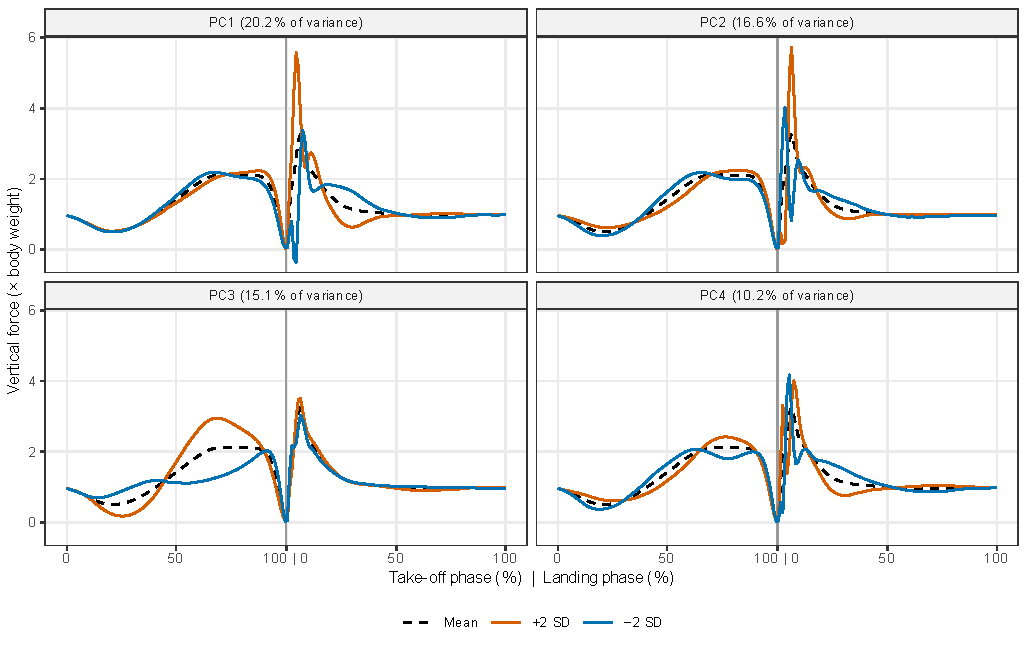
\includegraphics[width=\textwidth]{Fig6_pc_reconstructions_1s.pdf}
\caption{\capWindow}
\label{fig:window}
\end{figure}


\section{Discussion and implications}

\subsection{Principal findings}

This study asked whether countermovement jumps that score alike on conventional force-plate metrics also look alike, and how much of the shape of the force--time curve those metrics capture. Three findings stand out. First, when take-off and landing are analysed together, the dominant modes of variation lie in the landing, and the first describes how quickly the athlete arrests the fall. Second, jumps matched closely on jump height, or on relative peak force, were scarcely more alike in curve shape than jumps in general. Third, jump height, concentric peak force, eccentric braking impulse, early concentric impulse, age and body mass together explained no more than \rtwoPCC\% of the variance of any landing component, and less under cross-validation. Equal scores on these metrics therefore do not imply an equal jump. A further finding qualifies the interpretation of the components as strategies: most of their variance arose within athletes, between sessions and between trials of the same session.

\subsection{Comparison with previous work}

The results extend earlier evidence that discrete force-plate variables summarise the jump incompletely. \citet{dowling1993} found that no single kinetic or temporal variable explained vertical jump performance well, \citet{richter2014b} showed that dimensionality-reduction techniques captured performance-related features of the jump better than discrete points, and principal component waveform analysis has been used to identify the features of the curve associated with improvements in jump performance \citep{floria2019}. These studies, like most CMJ waveform analyses \citep{cormie2009,sole2018,harry2018}, examined the propulsive part of the jump and asked how curve features relate to performance. The present study reverses the question and asks how much of the curve the performance metrics account for; the matched-band analysis gives a direct and intuitive answer, because it holds jump height almost constant and observes what remains.

The sensitivity analysis clarifies where the unexplained variation lies. With the 1-s landing window a take-off component emerged that described the duration and amplitude of the propulsive force and was explained to about two-thirds by the conventional metrics. This agrees with the close relationships between contraction time, relative peak force, impulse and jump height that follow from impulse--momentum mechanics \citep{linthorne2001,mcmahon2018}, and with the distinction now drawn between performance metrics and strategy variables \citep{harry2024}. The metrics that practitioners usually report are therefore reasonable summaries of the take-off, but they are almost silent about the landing. This is not surprising, because the four vendor metrics describe propulsion, and the result should not be read as a failure of those metrics. Rather, it shows that the landing recorded in every trial contains substantial information that routine reports omit.

The importance of the landing is consistent with the wider literature. Landings that arrest the body quickly with high forces have been linked to injury risk in young female athletes \citep{leppanen2017}, and landing kinetics have some utility as predictors of injury \citep{pedley2020}. PC1, which separated short, stiff landings from longer, more compliant ones, corresponds closely to this construct. Its relation to landing duration follows from impulse--momentum: because the landing phase in the main analysis ends when the downward velocity reaches zero, the mean force over the phase is fixed by the touch-down velocity and the duration of the landing, so a shorter landing must be accompanied by higher forces. The weaker correlations with peak landing force indicate that the component describes the time course of force rather than its maximum alone.

\subsection{Trial-to-trial variability and the interpretation of strategies}

Between-athlete differences accounted for at most \betweenPCA\% of the variance of any component, which corresponds to poor single-trial reliability by conventional benchmarks \citep{koo2016}, and for PC2 to PC4 most of the variance arose between trials of the same session. The landing differences among jumps matched on jump height therefore reflect, to a large extent, how a given athlete landed on a given trial rather than a fixed characteristic of the athlete. This is in keeping with the view that movement variability is an intrinsic and often functional feature of skilled performance \citep{davids2003,bartlett2007,preatoni2013}, and with the known sensitivity of CMJ variables to the number of trials and to protocol details \citep{cormack2008,heishman2020}. Landing behaviour is also likely to depend on instructions and perceived effort \citep{hite2025}, which were not standardised for landing in routine testing. The word strategy should therefore be understood here as the way in which a trial was executed; whether athletes have stable landing strategies can be judged only from repeated, standardised landings.

\subsection{Methodological implications}

Two analytical choices had a large influence on the results and should be reported in any similar study. The first is the definition of the end of the landing. Ending the landing at the lowest point of the COM confines the landing block to impact absorption and makes landing timing comparable across trials; a fixed window spends most of the block on quiet standing and compresses the impact into a few points, which lowered the variance captured by four components from \cumFour\% to \cumFourS\% and changed the composition of the components. The second is the scaling of the curve. Covariance PCA of body-weight-normalised force gives weight to each part of the curve in proportion to its variance, and because landing forces are larger and more variable than take-off forces, the take-off contributes little to the leading components unless the landing is short or analysed separately. Neither choice is right or wrong, but they answer different questions, and the matched-band and regression results should be interpreted with them in mind. Alignment on further events, such as the landing force peak \citep{moudy2018}, functional PCA \citep{ramsay2005,warmenhoven2019} and statistical parametric mapping \citep{pataky2013} are natural extensions.

\subsection{Practical applications}

For practitioners, the results have four implications. First, two athletes with the same jump height may land very differently, so ranking or grouping athletes on jump height alone conceals differences in landing mechanics. Second, the landing is recorded in every CMJ at no additional cost, and simple landing descriptors, in particular landing duration to the lowest point of the COM and peak landing force relative to body weight, capture much of the dominant landing component and could be added to routine reports. Third, because landing shape varies considerably between trials, decisions should be based on the mean of several trials, or on repeated sessions, rather than on a single landing. Fourth, unusual landing curves should prompt closer observation of how an athlete lands, under standardised instructions, rather than a diagnosis; their relationship with injury in footballers has not been established.

\subsection{Strengths and limitations}

The strengths of the study include a large set of routinely collected trials analysed in full, the inclusion of the landing phase, a direct test of the equivalence of matched jumps, evaluation schemes that respect the repeated structure of the data, explicit sensitivity analyses of the main analytical choices, and a single script that reproduces every reported result from the de-identified data.

Several limitations should be noted. The landing was not standardised in routine testing, so part of its variation may reflect instructions, habits or effort rather than neuromuscular capacity. The end of the landing depends on the body mass and on a velocity estimated from flight time, both of which carry error \citep{street2001}, and could not be found in \nLowcomMissing{} trials. The sample comprised male footballers from a single centre over a wide age range (\ageMin--\ageMax{} years), most of them adolescents; maturity status was not recorded, although growth and maturation affect jump performance in youth athletes \citep{malina2015,lloyd2012}, and the results may not generalise to female athletes, other sports or other age groups. The regressions were linear and used four metrics; other vendor variables, including landing variables, would explain more of the landing components, and non-linear models might explain somewhat more, although the weak correlations suggest that the gain would be limited. PCA on linearly time-normalised curves combines differences in timing and in amplitude. Finally, the number of components was fixed in advance rather than chosen from the data, which avoids tuning but means that the remaining components, which together explained about a quarter of the variance, were not interpreted.

\subsection{Future work}

Future studies should test whether landing components are stable when landings are standardised and repeated, relate them to injury, fatigue and return-to-play outcomes in prospective designs, and examine female athletes and other sports. Separate analysis of the take-off and landing, registration on additional events and functional or multivariate methods that combine curve shape with timing would help to separate strategy from execution variability. Establishing reference values for landing components across age and maturity would make the information usable in routine monitoring.

\section{Conclusion}

In male footballers, countermovement jumps matched closely on jump height, or on relative peak force, differed almost as much in the shape of their force--time curves as jumps in general. The dominant differences lay in how athletes absorbed the landing, above all in how quickly the fall was arrested, and the four conventional vendor metrics, together with age and body mass, explained little of them. These differences were, however, largely trial-specific. The landing phase of the CMJ, which is recorded in every trial but rarely reported, adds information that conventional take-off metrics do not provide, and it deserves a place in routine force-plate reports, provided that it is interpreted over repeated trials.

\section*{Acknowledgements}
\todo{acknowledge the centre, coaches and athletes who provided the data, if permitted}

\section*{Disclosure statement}
The authors report there are no competing interests to declare. \todo{confirm}

\section*{Funding}
\todo{funding source and grant number, or state that no funding was obtained}

\section*{Data availability statement}
The de-identified trial data (curves and vendor metrics keyed by pseudonymous codes), the analysis script and all output tables are available in the project repository \todo{URL or DOI}. The raw ForceDecks exports and the key linking codes to athletes are not shared \todo{state the data owner and the terms under which raw data may be requested}.

\section*{Declaration of generative AI use}
\todo{The authors must state whether and how generative AI was used. Suggested wording, to be confirmed: an AI assistant was used to help write and run the analysis code and to draft the manuscript text; the authors reviewed all code, results and text and take full responsibility for the content.}

\bibliographystyle{tfapacite}
\bibliography{references}

\ifsubmission
\processdelayedfloats
\clearpage
\section*{Figure captions}
\noindent\textbf{Figure 1.} \capPipeline\par\medskip
\noindent\textbf{Figure 2.} \capMean\par\medskip
\noindent\textbf{Figure 3.} \capPCs\par\medskip
\noindent\textbf{Figure 4.} \capBand\par\medskip
\noindent\textbf{Figure 5.} \capRtwo\par\medskip
\noindent\textbf{Figure 6.} \capWindow\par
\fi
